\section{Agenti}

Gli agenti considerati nella modellazione di uno scenario rappresentante un supermercato sono diversi:

\begin{itemize}
    \item \textbf{Ostacoli} (Obstacles): rappresentano ostacoli fermi all'interno della mappa, zone non calpestabili dagli agenti in movimento.
    \item \textbf{Cassieri} (Cashiers): rappresentano i cassieri del supermercato, si posizionano alla cassa per servire i clienti, rimanendo nella loro posizione. Compaiono nello scenario quando la cassa apre e scompaiono quando la cassa chiude. Insieme a questi agenti vengono gestite le casse vere e proprie, ovvero i punti di pagamento a cui i clienti sono diretti prima di uscire dal supermercato. Queste casse rappresentano, come gli ostacoli, delle zone non calpestabili del terreno, ma contengono anche proprietà aggiuntive come il tempo per cui devono ancora rimanere aperte e lo stato attuale: aperta o chiusa. 
    \item \textbf{Clienti} (Customers): questi sono gli agenti che si muovono all'interno dell'area casse. Questi agenti possiedono diversi attributi utili all'esecuzione del proprio compito tra cui: numero di prodotti da acquistare, tempo necessario per fare la spesa, tempo di pagamento, stato attuale, prossima destinazione da raggiungere ecc...
    Nella modalità \textbf{snake} eseguono un compito molto semplice, ovvero quello di accodarsi e aspettare che gli venga assegnata una cassa una volta raggiunta la fine della coda. Nella modalità \textbf{classic}, invece, i clienti ricercano quella che è la soluzione che ritengono migliore per poter raggiungere una cassa disponibile nel minor tempo possibile, tenendo in considerazione diversi fattori tra cui la distanza da ogni cassa e il numero di persone nelle corrispondenti coda. 
\end{itemize}

Da questo momento in poi verranno analizzati quelli che sono gli aspetti più interessanti utilizzati per la gestione degli agenti. Nella trattazione successiva gli agenti considerati sono i Clienti (Customers), in quanto sono coloro che hanno la possibilità di muoversi e di accodarsi alle casse.

\subsection{Entrata all'area casse}

I clienti una volta terminata la spesa all'interno del supermercato, devono comparire nella zona casse, in modo da poter pagare e poi uscire dallo scenario. Nel supermercato modellato sono presenti 5 corsie, da ognuna delle quali si può giungere all'area casse. Lo spawn degli agenti nell'area casse viene quindi eseguito su una di queste 5 corsie, ma la distribuzione di probabilità di accedere all'area casse non sarà uniforme sulle 5 corsie in quanto sarà molto più probabile che una persona percorra tutte o quasi le corsie. Questo perché prodotti di categorie diverse sono in corsie differenti e spesso quando si va fare la spesa si ha la necessità di acquistare prodotti di vario tipo, unito al fatto che la disposizione degli scaffali e dei prodotti è simile nei vari supermercati, predeterminando il percorso dei clienti, e mostrandogli più prodotti di quelli che sarebbero inizialmente intenzionati ad acquistare. Sulla base di tali motivazioni è stata predisposta un probabilità del 35\% che un agente acceda alla zona casse dall'ultima corsia, del 25\% dalla penultima, del 20\% dalla terza ed infine del 10\% dalla seconda e dalla prima.  

\subsection{Fasi Agente}

Un cliente durante la sua permanenza all'interno del supermercato si trova in diverse fase, ad ognuna delle quali corrisponde un diverso obiettivo che l'agente deve perseguire. Naturalmente le fasi saranno leggermente differenti nelle due modalità di code. 

Nella figura sottostante vengono mostrate le fasi dell'agente nella modalità \textbf{classic}:

\begin{itemize}
    \item \textbf{Shopping}: il cliente si trova all'interno del supermercato e sta facendo la spesa. Essendo il supermercato gestito come una \textit{black-box} il cliente non viene mostrato durante questa fase, ma è conteggiato all'interno del grafico a torta che mostra la porzione di agenti in \textbf{Shopping}. Una volta che il cliente ha terminato di fare la spesa allora passa nello stato \textbf{Reaching the queue}.
    \item \textbf{Reaching the queue}: il cliente è appena comparso nella zona casse, in una delle 5 corsie, e valuta in base alla \textit{distanza} e al \textit{numero di altre persone in ogni coda} quale sia la scelta ottimale per minimizzare il tempo di attesa alle code. In questa fase si muove verso la destinazione prestabilita, avendo anche la possibilità di cambiare la propria decisione a fronte di variazioni della situazione circostante. Una volta raggiunta la coda entra nello stato \textbf{In queue}.
    \item \textbf{In queue}: in questo stato il cliente è fermo ed attende il proprio turno per essere servito. Ad ogni step l'agente si muove in avanti qualora la fila scorra e lasci libera una cella per il movimento. Una volta raggiunta la cassa corrispondente a tale coda il cliente passa nello stato di \textbf{Paying}.
    \item \textbf{Paying}: l'agente viene servito e una volta terminato il tempo di pagamento esce dalla scena.
\end{itemize}

\begin{figure}[h!]
    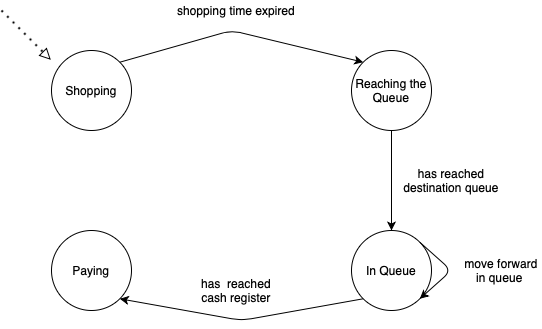
\includegraphics[width=\linewidth]{img/FSM-phases-classic.png}
    \centering
    \caption{\textit{Fasi cliente con coda \textbf{classic}.}}
\end{figure}

Nella figura sottostante vengono riportate le fasi attraversate dall'agente nella modalità \textbf{snake}. Di seguito verranno descritte solo quelle fasi che differiscono dal caso precedente:

\begin{itemize}
    \item \textbf{Shopping}.
    \item \textbf{Reaching the queue}: in questa fase il cliente si muove verso la destinazione, contrassegnata dalla posizione di inizio della coda a serpentone; una volta raggiunta la coda entra nello stato \textbf{In queue}.
    \item \textbf{In queue}: in questa fase il cliente si muove fino al fondo della coda (qualora ci siano altro agenti in attesa), e una volta raggiunta tale posizione rimane fermo in coda e si muove nel momento in cui i clienti che lo precederono muovono a loro volta in avanti. Rimane in questa fase fino al raggiungimento della posizione di fine della coda a serpentone, passando nello stato \textbf{Reaching Cashier}.
    \item \textbf{Reaching Cashier}: l'agente si trova in questa fase dal momento in cui raggiunge la testa del serpentone, mentre attende che una cassa si liberi e gli venga assegnata, fino a quando raggiunge una cassa per il pagamento (momento in cui passa nello stato \textbf{Paying}).
    \item \textbf{Paying}.
\end{itemize}

\begin{figure}[h!]
    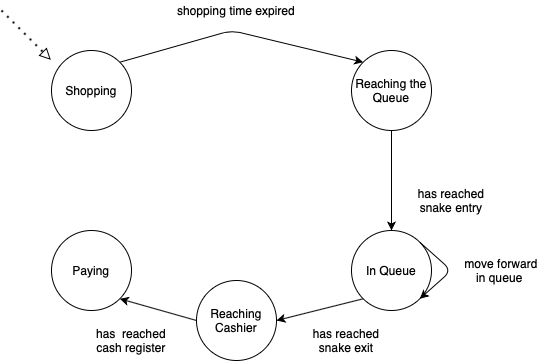
\includegraphics[width=\linewidth]{img/FSM-phases-snake.png}
    \centering
    \caption{\textit{Fasi cliente con coda \textbf{snake}.}}
\end{figure}

\subsection{Numero di Prodotti}

Un parametro importante che viene definito alla creazione dell'agente è il numero di prodotti che dovrà andare ad acquistare e che verrà utilizzato come base di partenza per il calcolo necessario a fare la spesa e per il tempo di pagamento. 

Questo parametro viene calcolato utilizzando una distribuzione normale con media e varianza espresse in funzione della capienza massima del supermercato, ovvero di 35 persone nella mappa utilizzata.

I parametri utilizzati per la normale sono $\mu = 35/2 = 17.5$ e $\sigma = 35/4 = 8.75$ scelti opportunamente dopo una fase di calibrazione e testing. 

Il numero di prodotti viene quindi ottenuto estraendo un campione da questa distribuzione normale, e arrotondandolo per eccesso, in quanto il numero di prodotti deve essere necessariamente intero.

La distribuzione ottenuta estraendo $100000$ campioni dalla normale con media e deviazione standard definiti sopra è quella riportata nella figura sottostante. 

\begin{figure}[h!]
    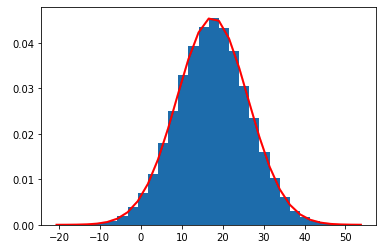
\includegraphics[width=\linewidth]{img/pcount-distribution.png}
    \centering
    \caption{Distribuzione normale con $\mu=17.5$ e $\sigma=8.75$.}
\end{figure}

\subsection{Shopping Time}

Alla creazione di un cliente, sulla base del numero di prodotti generato dalla distribuzione descritta precedentemente, viene calcolato quello che è lo \textit{shopping time}, ovvero il tempo che l'agente in questione impiegherà nella fase di \textbf{Shopping}, espresso in step. La stima di questo parametro rappresenta un'approssimazione del tempo impiegato dal cliente a fare la spesa all'interno del supermercato, ovvero dell'area da noi considerata come una \textbf{black-box}; a tal proposito l'agente non viene visualizzato nell'area casse durante questo periodo, in quanto impegnato nelle corsie del supermercato da noi non modellate. 

La formula utilizzata per calcolare questo tempo dipende dal parametro \textit{numero di prodotti} (\textit{product count}), nel seguente modo: 

\begin{equation*}
shopping time = 3 + product count * 0.75
\end{equation*}

Supponendo, ad esempio, che un cliente debba acquistare 20 prodotti, allora il tempo impiegato per fare la spesa sarà di circa 18 step.

\subsection{Paying Time}

Altro parametro che viene assegnato ad ogni cliente alla sua creazione è quello legato al tempo di pagamento (\textbf{paying time}). Questo parametro rappresenta il tempo che l'agente trascorrerà nella fase di \textbf{paying}, davanti alla cassa, in attesa di terminare il pagamento, per poi scomparire dalla scena. La stima di questo parametro rappresenta un'approssimazione del tempo impiegato dal cliente ad effettuare effettuare il pagamento; durante questo periodo il cliente sarà posizionato nella casella a fianco della cassa, in attesa di terminare il pagamento e andarsene. 

La formula utilizzata per calcolare questo tempo dipende sempre dal parametro \textit{numero di prodotti} (\textit{product count}), nel seguente modo:

\begin{equation*}
paying time = 1 + product count * 0.25
\end{equation*}

Supponendo, ad esempio, che un cliente debba acquistare 20 prodotti, allora il tempo impiegato per effettuare il pagamento una volta raggiunta la cassa sarà di circa 6 minuti.

\subsection{Scelta della destinazione}



